\documentclass[11pt, a4paper]{article}

% ── Packages ──────────────────────────────────────────────────────────────
\usepackage[top=2.5cm, bottom=2.5cm, left=3cm, right=3cm]{geometry}
\usepackage[utf8]{inputenc}
\usepackage[T1]{fontenc}
\usepackage{lmodern}
\usepackage{microtype}
\usepackage{graphicx}
\usepackage{booktabs}
\usepackage{amsmath}
\usepackage{xcolor}
\usepackage{listings}
\usepackage[font=small, labelfont=bf]{caption}
\usepackage{float}
\usepackage{parskip}
\usepackage[colorlinks=true, linkcolor=black, urlcolor=blue, citecolor=black]{hyperref}

% ── Python listing style ───────────────────────────────────────────────────
\definecolor{bg}{rgb}{0.97,0.97,0.97}
\definecolor{kw}{rgb}{0.13,0.29,0.53}
\definecolor{st}{rgb}{0.50,0.00,0.60}
\definecolor{cm}{rgb}{0.40,0.40,0.40}

\lstdefinestyle{py}{
  language        = Python,
  backgroundcolor = \color{bg},
  basicstyle      = \ttfamily\footnotesize,
  keywordstyle    = \color{kw}\bfseries,
  stringstyle     = \color{st},
  commentstyle    = \color{cm}\itshape,
  numberstyle     = \tiny\color{cm},
  numbers         = left,
  numbersep       = 8pt,
  breaklines      = true,
  showstringspaces= false,
  frame           = single,
  framerule       = 0.4pt,
  xleftmargin     = 18pt,
  tabsize         = 4,
  morekeywords    = {True, False, None},
}
\lstset{style=py}

% ── Title page ─────────────────────────────────────────────────────────────
\begin{document}

\begin{titlepage}
  \centering
  \vspace*{1.5cm}

  
\includegraphics[width=4cm]{usilogo.png}\\[1.2cm]

  {\LARGE\scshape Università della Svizzera italiana}\\[0.3cm]
  {\large Faculty of Informatics}\\[2.5cm]

  \rule{\linewidth}{1pt}\\[0.5cm]
  {\Huge\bfseries Schelling's Model\\[0.3cm]of Segregation}\\[0.5cm]
  {\Large Homework 1 --- Particle Methods}\\[0.4cm]
  \rule{\linewidth}{1pt}\\[2.5cm]

  {\large\itshape Student}\\[0.3cm]
  {\Large\textbf{[Your Name]}}\\[0.5cm]
  {\large [Student ID]}\\[3cm]

  {\large Spring Semester 2026}\\[0.2cm]
  {\large Due: 10 March 2026}

  \vfill
\end{titlepage}

\tableofcontents
\newpage

% ══════════════════════════════════════════════════════════════════════════
\section{Introduction}
% ══════════════════════════════════════════════════════════════════════════

In 1971, Thomas Schelling showed that strong spatial segregation can emerge from
surprisingly mild individual preferences \cite{schelling1971}.
In his model, agents of two types (representing people of different social groups) live on
a grid. Each agent checks how many of its neighbours share the same type.
If this count is below a personal threshold~$H$, the agent is \emph{unhappy} and moves
to a new empty cell.
Even when each agent only requires a small number of similar neighbours to be satisfied,
the collective result is a city that is almost completely segregated.

This report presents a Python implementation of Schelling's model on a 100\,×\,100
toroidal grid.
In Part~A we compare four combinations of update order and movement direction at fixed
threshold $H = 4$.
In Part~B we fix the best strategy from Part~A and vary $H$ from 1 to 8, identifying
a sharp phase transition in the system's behaviour.

% ══════════════════════════════════════════════════════════════════════════
\section{Model Description}
% ══════════════════════════════════════════════════════════════════════════

\subsection{Grid and Initial Conditions}

The simulation uses a square grid of side $N = 100$, giving 10\,000 cells in total.
We place exactly 4\,500 Red agents (45\,\%), 4\,500 Blue agents (45\,\%), and
1\,000 empty cells (10\,\%) at uniformly random positions.
Table~\ref{tab:params} summarises the parameters.

\begin{table}[H]
  \centering
  \caption{Simulation parameters.}
  \label{tab:params}
  \begin{tabular}{ll}
    \toprule
    Parameter            & Value \\
    \midrule
    Grid size            & $100 \times 100 = 10\,000$ cells \\
    Red agents           & 4\,500 \ (45\,\%) \\
    Blue agents          & 4\,500 \ (45\,\%) \\
    Empty cells          & 1\,000 \ (10\,\%) \\
    Boundary conditions  & Periodic (toroidal) \\
    Neighbourhood        & Moore, radius 1 (8 adjacent cells) \\
    \bottomrule
  \end{tabular}
\end{table}

A typical initial configuration is shown in Figure~\ref{fig:initial}: the two agent
types are mixed uniformly and no spatial structure is visible.

\begin{figure}[H]
  \centering
  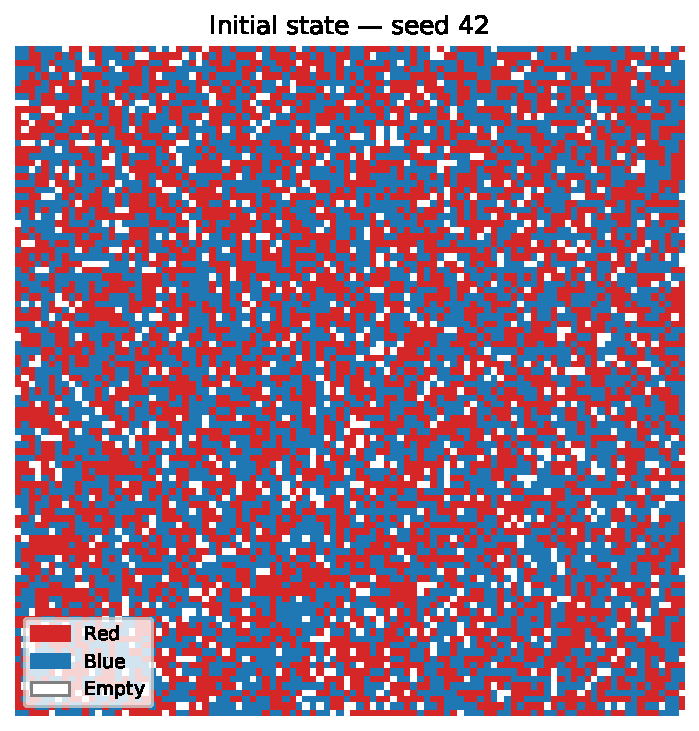
\includegraphics[width=0.42\linewidth]{figures/initial_state.pdf}
  \caption{Random initial configuration (seed 42). Red and Blue agents are fully mixed;
  no clusters are visible.}
  \label{fig:initial}
\end{figure}

\subsection{Periodic Boundary Conditions}

The grid is toroidal: the left edge connects to the right edge, and the top edge to the
bottom. This is implemented with modulo arithmetic, so every cell always has exactly
8 neighbours regardless of its position:

\begin{equation}
  r_{\text{nbr}} = (r + \Delta r) \bmod N,
  \qquad
  c_{\text{nbr}} = (c + \Delta c) \bmod N.
  \label{eq:pbc}
\end{equation}

\subsection{Happiness Condition}

An agent at position $(r, c)$ of type $s_{r,c}$ is \emph{happy} if at least $H$ of its
8 Moore neighbours share the same type:

\begin{equation}
  \sum_{(\Delta r,\,\Delta c)\;\in\;\mathcal{N}}
  \mathbf{1}\!\left[s_{\,(r+\Delta r)\%N,\,(c+\Delta c)\%N} = s_{r,c}\right] \geq H.
  \label{eq:happy}
\end{equation}

Empty cells are \emph{not} counted toward the threshold. An agent with only empty
neighbours has a count of zero and is therefore unhappy for any $H \geq 1$.

% ══════════════════════════════════════════════════════════════════════════
\section{Part A --- Comparing Four Strategies ($H = 4$)}
% ══════════════════════════════════════════════════════════════════════════

\subsection{Strategies}

In each iteration every agent is visited once.
If the agent is unhappy, it moves to the nearest empty cell in a chosen direction.
We test two choices of \emph{update order} and two choices of \emph{movement direction},
giving four combinations (Table~\ref{tab:combos}).

\begin{table}[H]
  \centering
  \caption{The four strategy combinations tested in Part~A with $H = 4$.}
  \label{tab:combos}
  \begin{tabular}{p{1.5cm} p{3.5cm} p{7cm}}
    \toprule
    Label  & Update order      & Movement direction \\
    \midrule
    RO-H   & Row-by-row        & Horizontal: pick left or right at random, move to
                                 the nearest empty cell in that row. \\[4pt]
    RO-RD  & Row-by-row        & Random direction: pick up/down/left/right at random,
                                 move to the nearest empty cell along that line. \\[4pt]
    RS-H   & Random sequence   & Horizontal (same as above). \\[4pt]
    RS-RD  & Random sequence   & Random direction (same as above). \\
    \bottomrule
  \end{tabular}
\end{table}

\textbf{Row-by-row order.} Agents are visited from left to right, top to bottom (standard
reading order). This is obtained naturally by enumerating occupied cells with
\texttt{numpy.where}, which returns indices in C (row-major) order.

\textbf{Random order.} The list of agent positions is shuffled before each iteration
using a separate random-number generator.

In both movement strategies, the agent moves to the first empty cell found in the chosen
direction, regardless of whether that position makes it happy.

Each combination is run with three different random seeds (42, 123, 777) to assess
variability.

\subsection{Results}

\begin{table}[H]
  \centering
  \caption{Number of iterations to reach full happiness ($H = 4$, max.\ 500 iterations).
  A ``$>$500'' entry means the simulation did not converge.}
  \label{tab:results_a}
  \begin{tabular}{lccc}
    \toprule
    Strategy & Seed 42 & Seed 123 & Seed 777 \\
    \midrule
    RO-H  & $>500$ & $>500$ & $>500$ \\
    RO-RD & 115    & 166    & 100    \\
    RS-H  & $>500$ & $>500$ & $>500$ \\
    RS-RD & \textbf{59}  & \textbf{75}  & \textbf{81}  \\
    \bottomrule
  \end{tabular}
\end{table}

\begin{figure}[H]
  \centering
  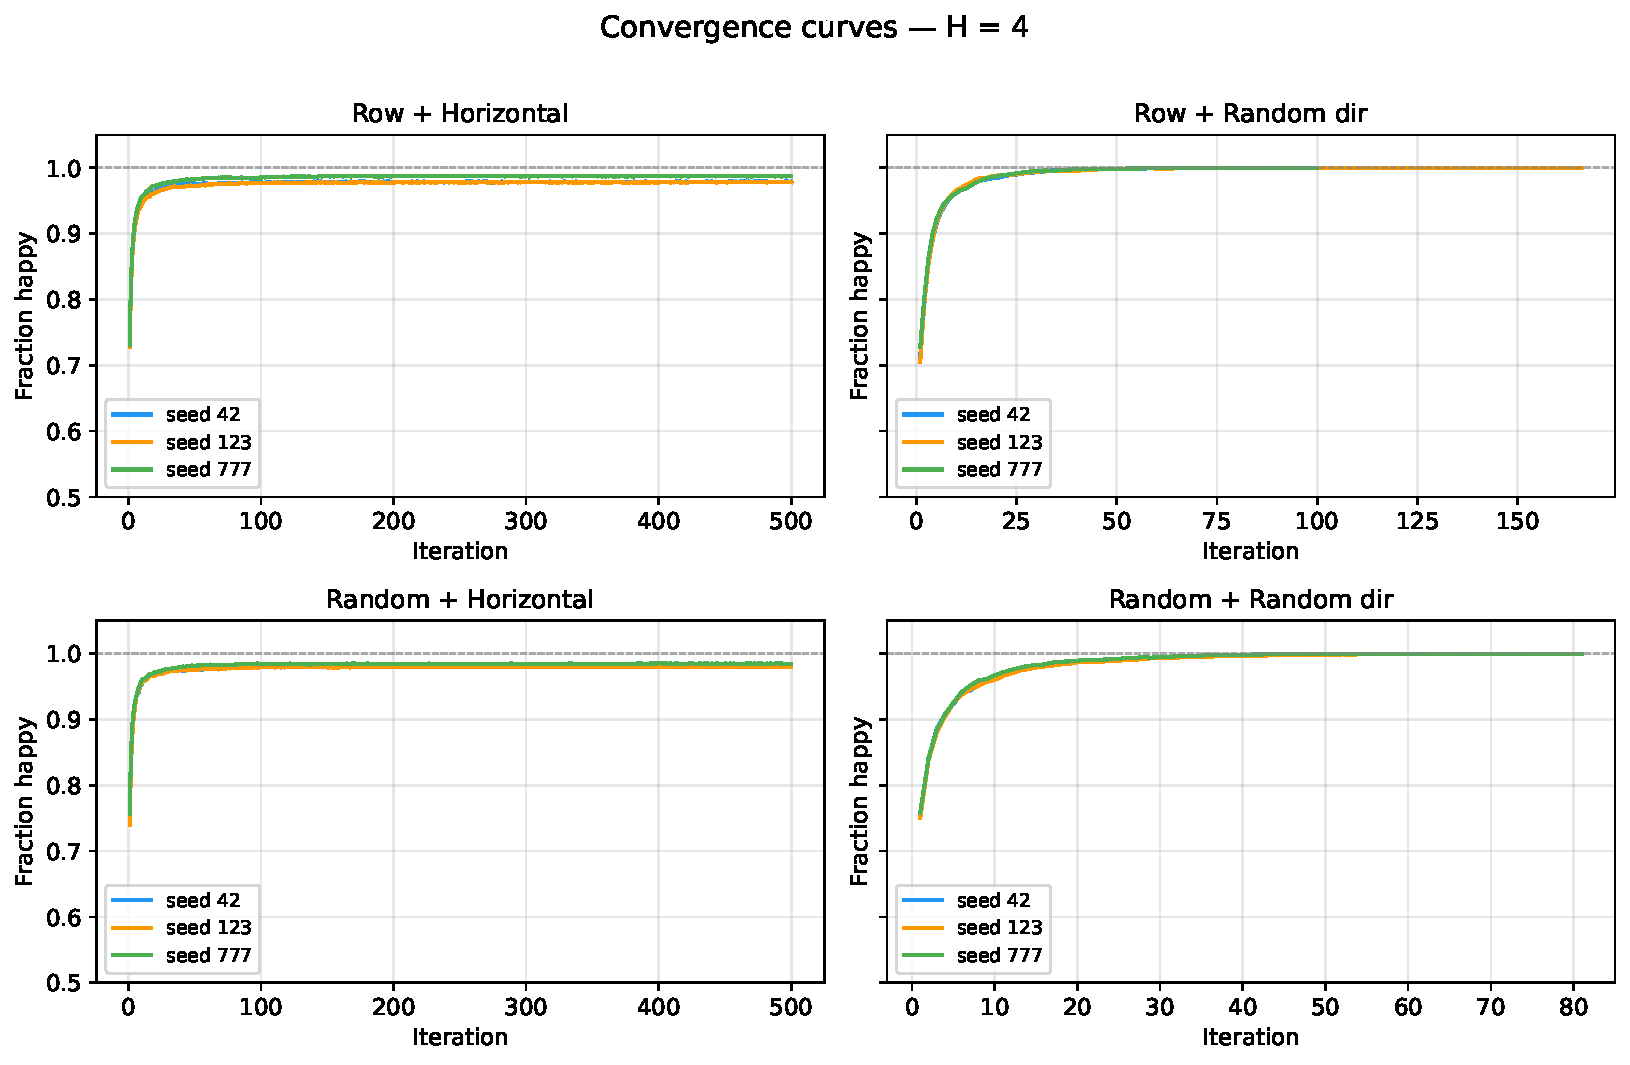
\includegraphics[width=\linewidth]{figures/convergence_curves.pdf}
  \caption{Fraction of happy agents per iteration for each strategy ($H = 4$, three seeds
  per panel). The two horizontal strategies (RO-H, RS-H) never reach 100\,\%; their
  curves plateau below the dashed line at 1.0. Both random-direction strategies converge,
  with RS-RD being the fastest.}
  \label{fig:conv_a}
\end{figure}

\begin{figure}[H]
  \centering
  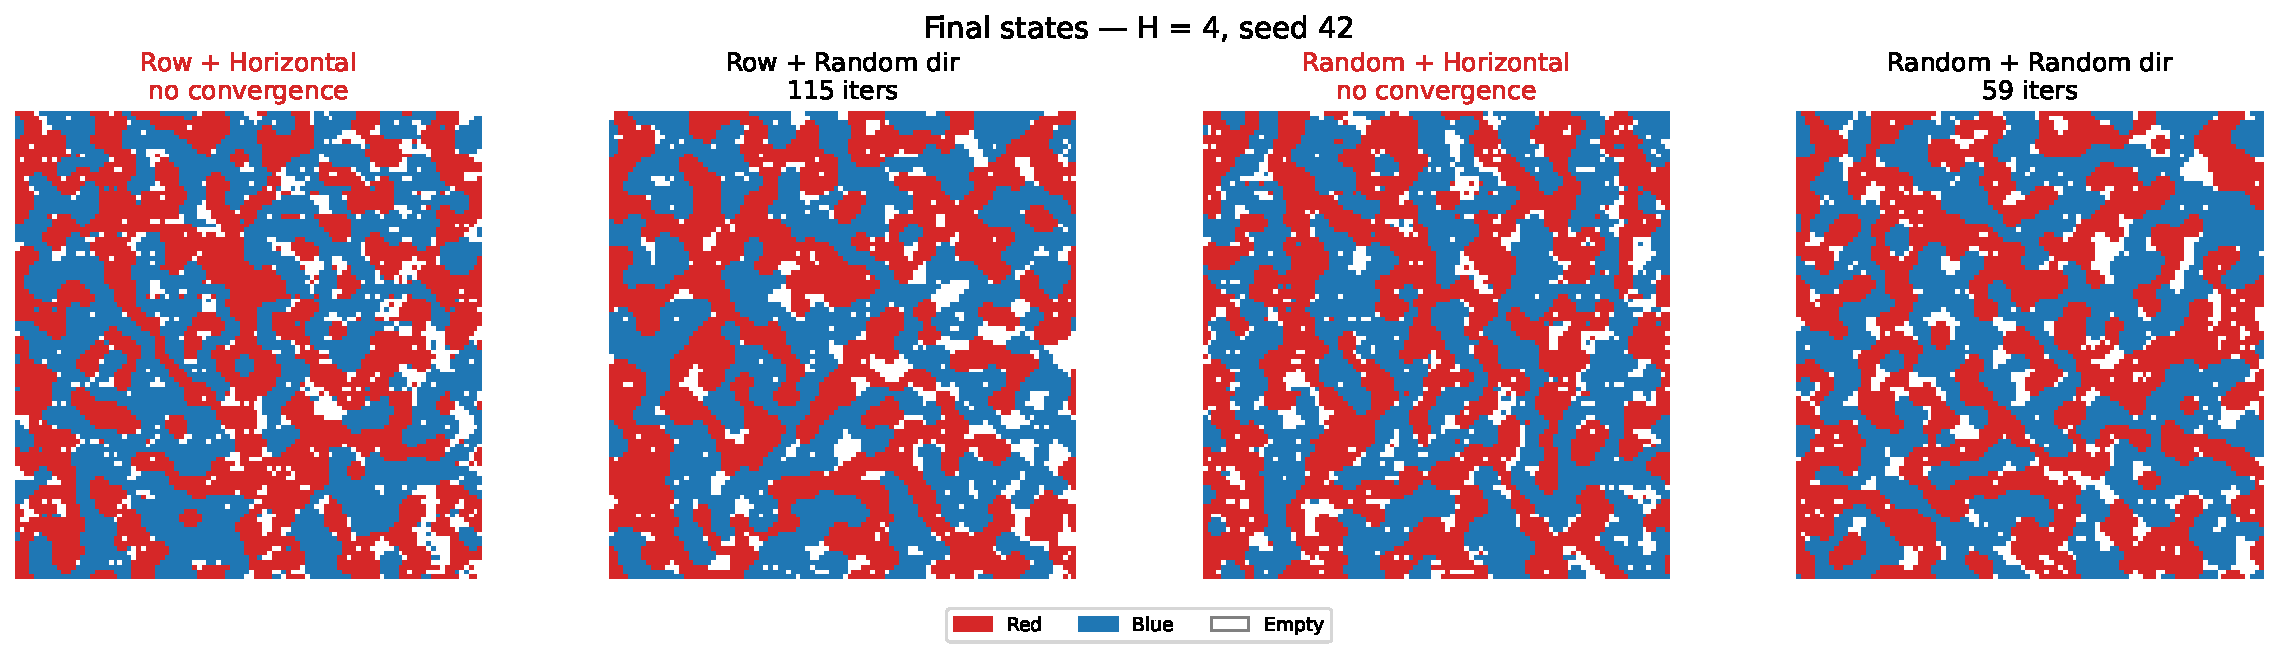
\includegraphics[width=\linewidth]{figures/final_states_a.pdf}
  \caption{Final grid states for seed 42 ($H = 4$). Titles in red indicate
  non-convergence. RO-H and RS-H show clear horizontal stripes (an artifact of
  left/right-only movement). RO-RD and RS-RD produce natural-looking segregated clusters.}
  \label{fig:final_a}
\end{figure}

\subsection{Discussion}

\paragraph{Why horizontal movement fails.}
When an agent can only move left or right, it cannot resolve mismatches with neighbours
directly above or below.
Two agents of opposite types sharing a vertical border will repeatedly trade positions
along their row, creating an oscillating cycle that never ends.
This produces the visible horizontal stripes in Figure~\ref{fig:final_a} and explains
why RO-H and RS-H never converge.

\paragraph{Effect of update order.}
With random-direction movement, random order (RS-RD, 59--81 iterations) converges
roughly twice as fast as row-by-row order (RO-RD, 100--166 iterations).
Row-by-row processing creates wave-like disturbances that propagate through the grid
before the next iteration, which slows down the overall dynamics.

\paragraph{Best strategy.}
\textbf{RS-RD (random order + random direction)} is the best combination: fastest
convergence, no artifacts.

% ══════════════════════════════════════════════════════════════════════════
\section{Part B --- Varying the Happiness Threshold ($H = 1$ to $8$)}
% ══════════════════════════════════════════════════════════════════════════

\subsection{Setup}

Using the best strategy from Part~A (RS-RD), we run simulations for each integer value
of $H$ from 1 to 8 with a maximum of 1\,000 iterations and the same three random seeds.

\subsection{Results}

\begin{table}[H]
  \centering
  \caption{Iterations to convergence for $H = 1$ to $8$ (RS-RD). ``$>$1000'' means no
  convergence within 1\,000 iterations.}
  \label{tab:results_b}
  \begin{tabular}{lccc}
    \toprule
    $H$ & Seed 42 & Seed 123 & Seed 777 \\
    \midrule
    1 & 5        & 2        & 2        \\
    2 & 12       & 8        & 13       \\
    3 & 36       & 38       & 44       \\
    4 & 105      & 89       & 80       \\
    5 & $>1000$  & $>1000$  & $>1000$  \\
    6 & $>1000$  & $>1000$  & $>1000$  \\
    7 & $>1000$  & $>1000$  & $>1000$  \\
    8 & $>1000$  & $>1000$  & $>1000$  \\
    \bottomrule
  \end{tabular}
\end{table}

\begin{figure}[H]
  \centering
  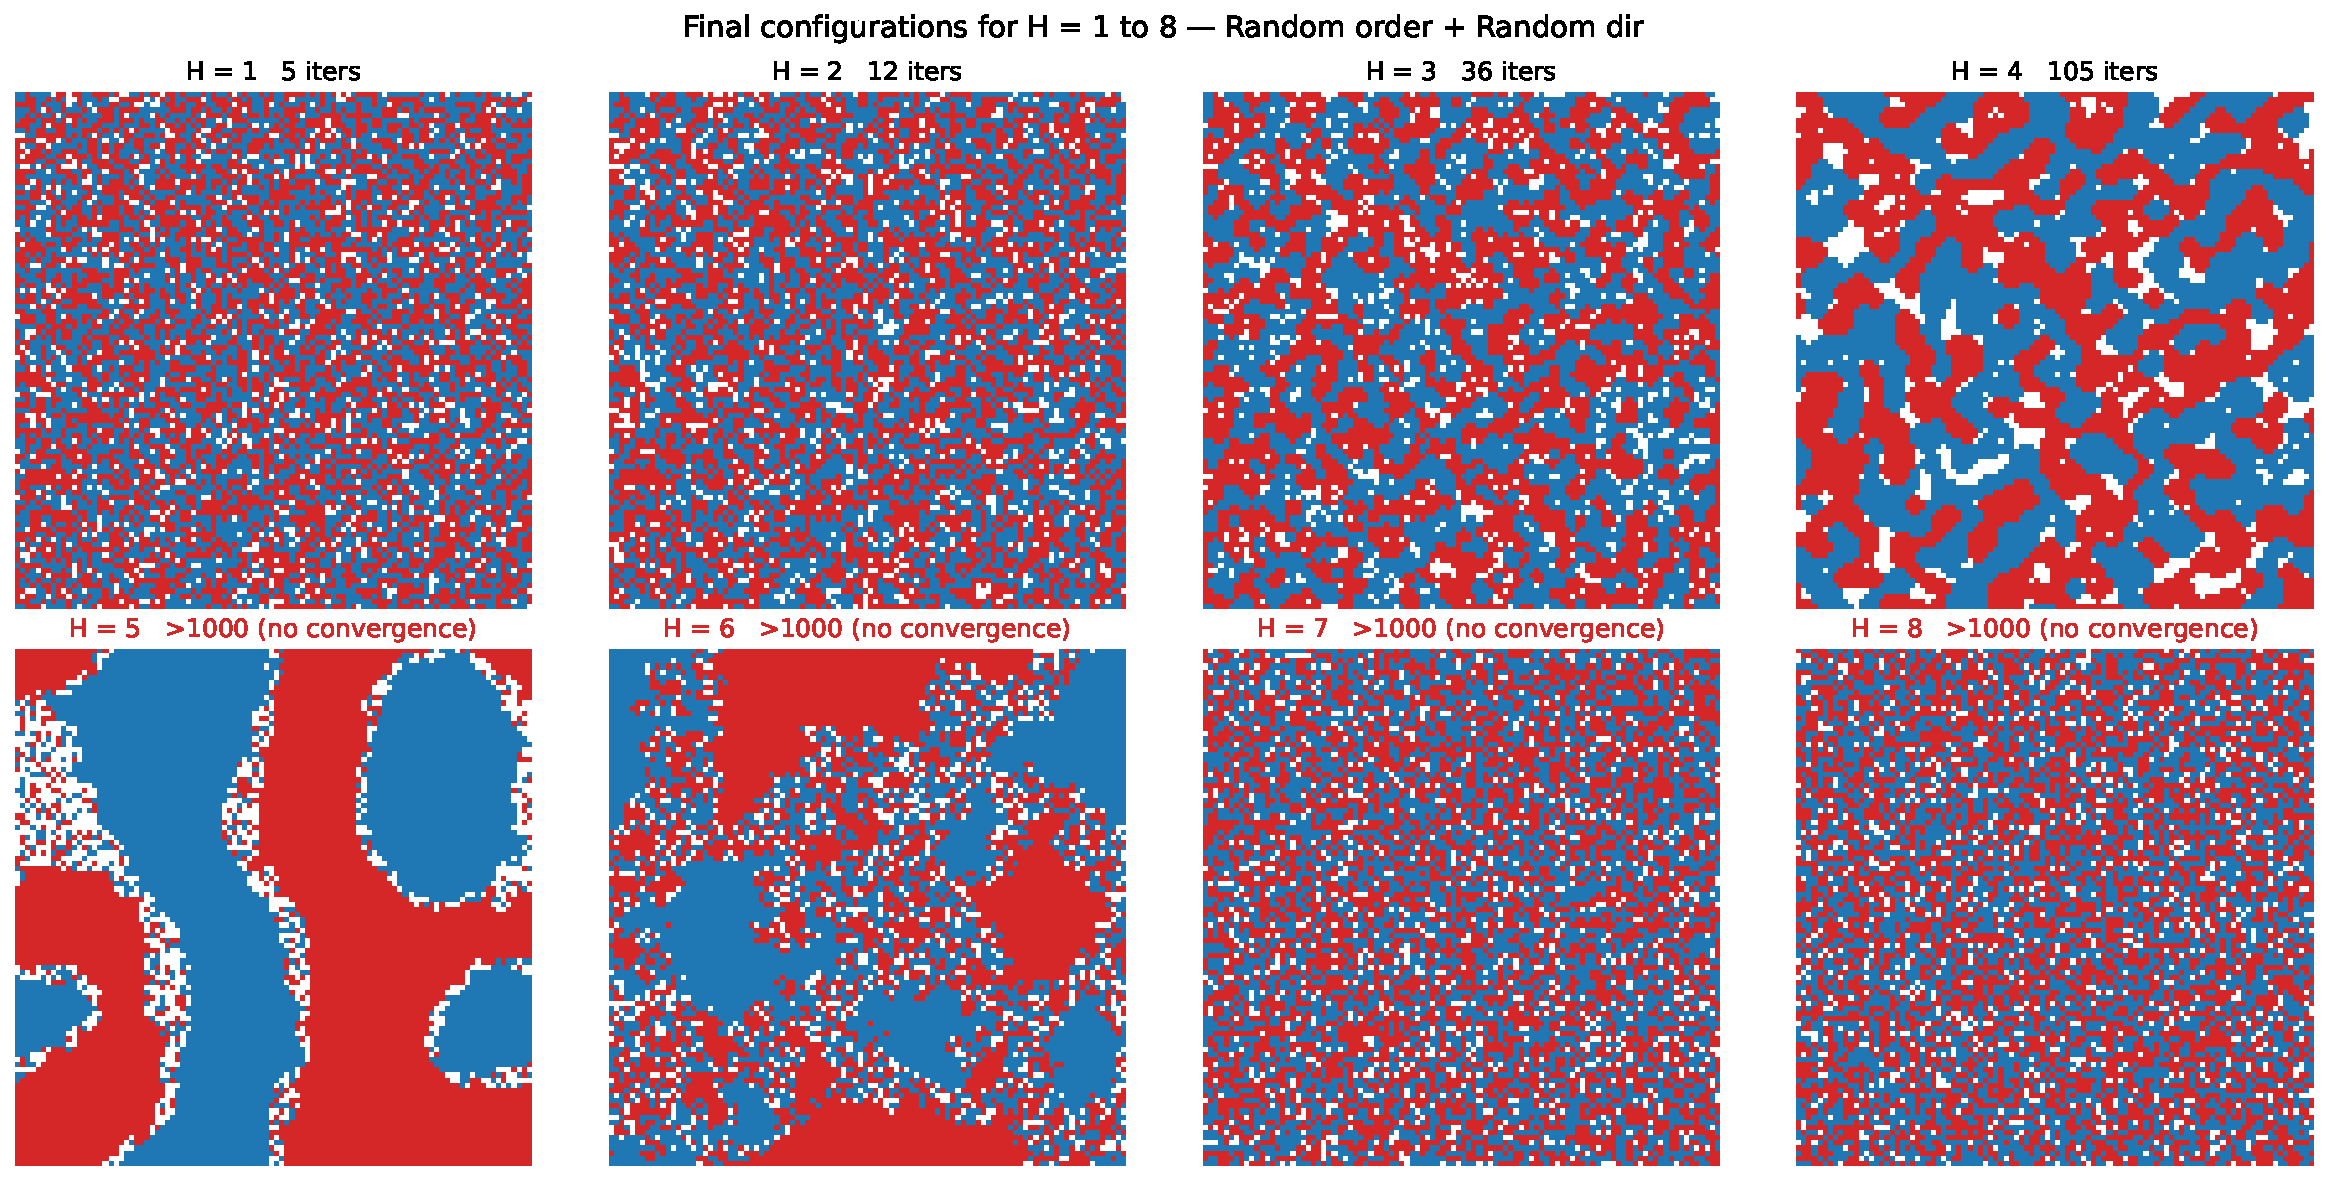
\includegraphics[width=\linewidth]{figures/final_states_h.pdf}
  \caption{Final configurations for $H = 1$ to $8$ (seed 42, RS-RD strategy). For
  $H \leq 4$ the system reaches full happiness, with clusters becoming larger and more
  compact as $H$ increases. For $H \geq 5$ (titles in red) no convergence is reached
  and the grid remains disordered.}
  \label{fig:final_h}
\end{figure}

\begin{figure}[H]
  \centering
  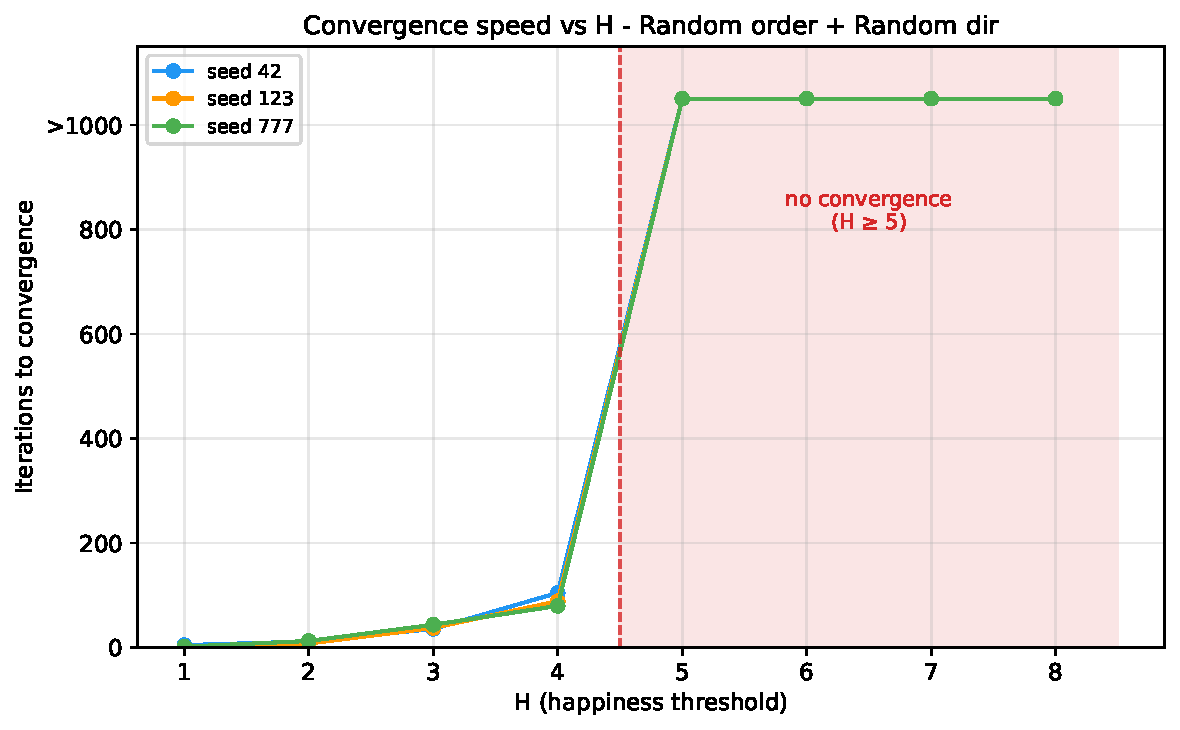
\includegraphics[width=0.75\linewidth]{figures/iterations_vs_h.pdf}
  \caption{Number of iterations to convergence as a function of $H$. For $H \leq 4$
  convergence time grows rapidly with $H$. The red shaded region ($H \geq 5$) marks
  values where no convergence was observed within 1\,000 iterations.}
  \label{fig:iters_h}
\end{figure}

\subsection{Phase Transition at $H = 4 \to 5$}

There is a sharp transition between $H = 4$ (always converges) and $H = 5$ (never
converges within 1\,000 iterations).

\paragraph{Geometric explanation.}
Each agent has 8 Moore neighbours. With 45\,\% Red and 45\,\% Blue and only 10\,\%
empty cells, an agent sitting at the boundary of a cluster typically has 3--5 neighbours
of the opposite type.
At $H = 5$, boundary agents need 5 same-type neighbours out of 8 --- but they share too
many cells with the opposite cluster, so this condition can never be satisfied
simultaneously for all boundary agents.
The system becomes trapped in a permanent non-equilibrium state where some agents are
always unhappy and keep moving.

At $H = 4$ the geometry still allows every agent to find a position with at least 4
same-type neighbours, so convergence is always possible.

\paragraph{Effect of $H$ on cluster structure.}
For $H \leq 4$, higher thresholds produce tighter, more clearly defined clusters (visible
in Figure~\ref{fig:final_h}): agents with a higher $H$ require more same-type neighbours
to stop moving, so they push deeper into existing clusters.
At $H = 1$ the clusters are loose and barely visible; at $H = 4$ they are large and
compact.

% ══════════════════════════════════════════════════════════════════════════
\section{Conclusion}
% ══════════════════════════════════════════════════════════════════════════

We implemented Schelling's model on a 100\,×\,100 toroidal grid and studied how update
strategies and the happiness threshold $H$ affect segregation dynamics.

\begin{itemize}
  \item \textbf{Horizontal-only movement prevents convergence.} Agents cycling left and
    right along rows cannot resolve vertical neighbourhood conflicts, creating
    oscillations that never end.
  \item \textbf{Random order is faster than row-by-row order.} With random-direction
    movement, random order converges roughly twice as fast by avoiding row-propagation
    artefacts.
  \item \textbf{Best strategy: RS-RD} (random order + random direction), converging in
    59--81 iterations for $H = 4$.
  \item \textbf{Phase transition at $H = 4 \to 5$.} Below this threshold the system
    always reaches full happiness; above it the geometric constraints of the 45/45/10
    population make full happiness impossible.
\end{itemize}

% ══════════════════════════════════════════════════════════════════════════
\begin{thebibliography}{9}
  \bibitem{schelling1971}
    T.\,C.\ Schelling,
    \textit{Dynamic Models of Segregation},
    Journal of Mathematical Sociology, 1(2), 143--186, 1971.
\end{thebibliography}

% ══════════════════════════════════════════════════════════════════════════
\appendix
\section{Source Code}
% ══════════════════════════════════════════════════════════════════════════

All code is in Python\,3 using NumPy and Matplotlib. The full notebook (\texttt{hw1.ipynb})
is included alongside this report. Below we list the core simulation functions; plotting
code is in the notebook.

% ── Setup ─────────────────────────────────────────────────────────────────
\subsection*{A.1 \quad Constants and Grid Initialisation}

\begin{lstlisting}
import numpy as np

N = 100
EMPTY, RED, BLUE = 0, 1, 2
OFFSETS = [(-1,-1), (-1,0), (-1,1), (0,-1), (0,1), (1,-1), (1,0), (1,1)]

def init_grid(seed=None):
    rng  = np.random.default_rng(seed)
    n    = N * N
    nr, nb = int(0.45*n), int(0.45*n)
    flat = np.array([RED]*nr + [BLUE]*nb + [EMPTY]*(n-nr-nb), dtype=np.int8)
    rng.shuffle(flat)
    return flat.reshape(N, N)
\end{lstlisting}

% ── Happiness ─────────────────────────────────────────────────────────────
\subsection*{A.2 \quad Happiness Functions}

\texttt{happy\_map} uses \texttt{numpy.roll} to shift the entire grid by one cell in
each of the eight Moore directions and count same-type neighbours in a single vectorised
pass (periodic BC is automatic since \texttt{roll} wraps by default).
\texttt{is\_happy} does the same check for a single cell and is used during the
per-agent loop.
\texttt{frac\_happy} calls \texttt{happy\_map} for the fast termination check.

\begin{lstlisting}
def happy_map(grid, H):
    # count same-type neighbours for every cell at once (vectorised)
    same = np.zeros_like(grid, dtype=np.int8)
    for dr, dc in OFFSETS:
        nbr = np.roll(np.roll(grid, -dr, axis=0), -dc, axis=1)
        same += ((nbr == grid) & (grid != EMPTY)).astype(np.int8)
    return (grid == EMPTY) | (same >= H)

def is_happy(grid, r, c, H):
    if grid[r, c] == EMPTY:
        return True
    same = sum(grid[(r+dr)%N, (c+dc)%N] == grid[r, c] for dr, dc in OFFSETS)
    return same >= H

def frac_happy(grid, H):
    hmap = happy_map(grid, H)
    return float(hmap[grid != EMPTY].mean())
\end{lstlisting}

% ── Movement ──────────────────────────────────────────────────────────────
\subsection*{A.3 \quad Movement Functions}

\begin{lstlisting}
def move_horizontal(grid, r, c, rng):
    step = int(rng.integers(0, 2)) * 2 - 1   # -1 (left) or +1 (right)
    for k in range(1, N):
        nc = (c + k*step) % N
        if grid[r, nc] == EMPTY:
            return (r, nc)
    return None

def move_random_dir(grid, r, c, rng):
    d = int(rng.integers(0, 4))               # 0=up 1=down 2=left 3=right
    if   d == 0: seq = [((r-k)%N, c)        for k in range(1, N)]
    elif d == 1: seq = [((r+k)%N, c)        for k in range(1, N)]
    elif d == 2: seq = [(r,        (c-k)%N) for k in range(1, N)]
    else:        seq = [(r,        (c+k)%N) for k in range(1, N)]
    for nr, nc in seq:
        if grid[nr, nc] == EMPTY:
            return (nr, nc)
    return None
\end{lstlisting}

% ── Simulation ────────────────────────────────────────────────────────────
\subsection*{A.4 \quad Simulation Engine}

\texttt{run\_iter} processes agents in the chosen order.
\texttt{numpy.where} returns occupied positions in C (row-major) order by default,
which gives row-by-row traversal for free.
For random order, the list is shuffled in-place before the loop.

\begin{lstlisting}
def run_iter(grid, H, order, movement, rng):
    rows, cols = np.where(grid != EMPTY)
    pos = list(zip(rows.tolist(), cols.tolist()))
    if order == 'random':
        rng.shuffle(pos)
    move = move_horizontal if movement == 'horizontal' else move_random_dir
    for r, c in pos:
        if not is_happy(grid, r, c, H):
            t = move(grid, r, c, rng)
            if t:
                grid[t] = grid[r, c]
                grid[r, c] = EMPTY

def run_sim(g0, H, order, movement, max_iter=500, seed=None):
    grid = g0.copy()
    rng  = np.random.default_rng(seed)
    hist = []
    for _ in range(max_iter):
        run_iter(grid, H, order, movement, rng)
        f = frac_happy(grid, H)
        hist.append(f)
        if f >= 1.0:
            return grid, len(hist), hist
    return grid, None, hist
\end{lstlisting}

\end{document}
